\section{Presenting the HH to 4b analysis} \label{section: HH4b}

\subsection{Aim of the HH to 4b analysis}

As mentioned in the Introduction (Section \ref{intro}) we introduce the the Brout–Englert–Higgs mechanism that allows to generate the masses of vector bosons without breaking the gauge invariance explicitly. This mechanism introduces the Higgs field $H$, a real scalar field with which massive particles interact to acquire mass. The Higgs boson is an excitation of this field, therefore its discovery by the ATLAS and CMS experiments proves the existence of a scalar field in the SM of particle physics. Nevertheless, to further probe this mechanism, we want to verify the shape of the Higgs potential postulated by the Higgs mechanism. As shown in Eq.(\ref{eq:Higgs potential}), the shape of this potential is governed by the parameter $\lambda$.

\begin{equation}
    V(\Phi^\dag \Phi)=-\mu^2 \Phi^\dag \Phi + \lambda (\Phi^\dag \Phi)^2
    \label{eq:Higgs potential}
\end{equation}

\noindent where $\Phi$, when parameterized in terms of a particular gauge, is the real scalar field that introduces the Higgs field:

\begin{equation}
    \Phi= \frac{1}{\sqrt{2}}\bigg( {0 \atop v + H} \bigg)
\end{equation}

\noindent where $H$ is the Higgs field and $v=\sqrt{\frac{\mu^2}{\lambda}}$. After the EWSB, the Higgs potential in the SM Lagrangian is written as follows \cite{higgs_potential}:

\begin{equation}
    V(H)= \frac{1}{2} m_H^2 H^2 + \lambda v H^3 +\frac{1}{4} \lambda H^4 + \frac{\lambda}{4} v^4
    \label{eq: higss pot after EWSB}
\end{equation}

\noindent the first term corresponds to the mass term of the Lagrangian as it contains the Higgs boson mass and the last term corresponds to the vacuum energy density. The second and third terms correspond to the three-point and four-point self-interaction terms respectively. As can be observed in Eq.(\ref{eq: higss pot after EWSB}), the self-interaction terms are proportional to $\lambda$, the Higgs boson self-coupling constant. Therefore, by experimentally measuring the Higgs self-coupling it is possible to probe the shape of the scalar potential.

In order to measure this self-coupling there are currently two complementary strategies:
\begin{itemize}
    \item Direct measurements of di-Higgs (HH), which are theoretically clean but experimentally challenging due to the low cross-section of this process.
    \item Indirect measurements in single Higgs, which needs more complicated theoretical assumptions but experimentally has more statistics as the single Higgs cross-section is around 1000 times larger than the di-Higgs production cross-section.
\end{itemize}

In the following sections, the focus will be only on the direct measurements of HH. In particular, by measuring the HH cross-section it is possible to get information on $\lambda$ as the latter can be parameterized in terms of anomalous Higgs boson couplings $\kappa_\lambda$, where $\kappa_\lambda$ is defined as follows:

\begin{equation}
    \kappa_\lambda=\frac{\lambda_{HHH}}{\lambda^{SM}_{HHH}}
\end{equation}


The dominant HH production modes in the SM are:
\begin{itemize}
    \item Gluon-gluon fusion (ggF) with a cross section $\sigma^{\text{ggF}}_{\text{HH}}=31.1^{+2.1\%}_{-7.2\%}$ fb at $\sqrt{s}=13$TeV (add Feynman diagrams?)
    \item Vector-boson fusion (VBF) with a cross section $\sigma^{\text{VBF}}_{\text{HH}}= 1.726 \pm 0.036$ fb at $\sqrt{s}=13$TeV (add Feynman diagrams?)
\end{itemize}


The branching ratios (BR) of the Higgs boson are shown in Figure \ref{fig: BR Higgs}. As can be observed in the Figure, for $m_H=125$GeV the highest BR is given by the $H\to b\Bar{b}$ channel. Nevertheless, proton-proton collisions occur at the LHC, therefore we have a high QCD background of multijet production, hence this channel's low signal/background ratio (S/B). However, even considering the low S/B of this process, since the HH cross section is so small we will be interested in the $HH \to 4b$ channel, as it has the highest BR.

\begin{figure}[hbt]
    \centering
    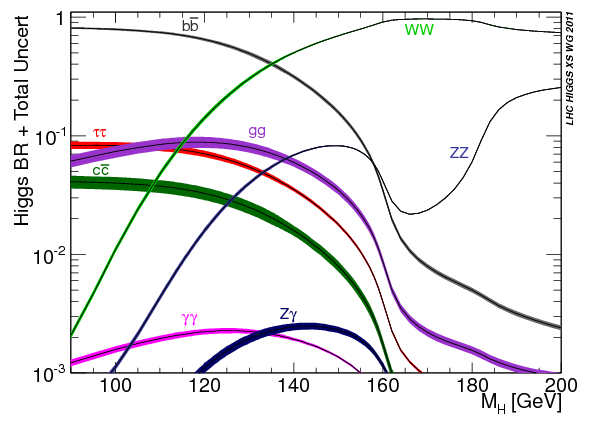
\includegraphics[width=0.7\linewidth]{Images/4.HH4b Analysis/Higgs intro/BR_higgs.png}
    \caption{Branching ratios and their uncertainties of the Higgs boson decay channels as a function oh the Higgs mass $M_H$ (cite)}
    \label{fig: BR Higgs}
\end{figure}

There are two main $HH \to 4b$ types of searches:
\begin{itemize}
    \item Resolved searches, where each $b$ quark is reconstructed as separate jets with radius (R=0.4)
    \item Boosted searches, where the $H\to bb$ decay is reconstructed as a single large-radius jet (R=0.8 or 1)
\end{itemize}

In the following sections, the focus will be on resolved searches for ggF HH production mechanism in the $b\Bar{b}b\Bar{b}$ decay channel.

\newpage

\subsubsection{Signature}
Figure \ref{fig: topology} shows the topology of the $HH\to 4b $ decay. As can be observed, we have 4 b quarks in our final state. These b quarks will then hadronize into B hadrons and will be detected as jets in the detector. Therefore, the signature expected in the detector is four small-radius b-jets (R=0.4)
\begin{figure}[hbt]
    \centering
    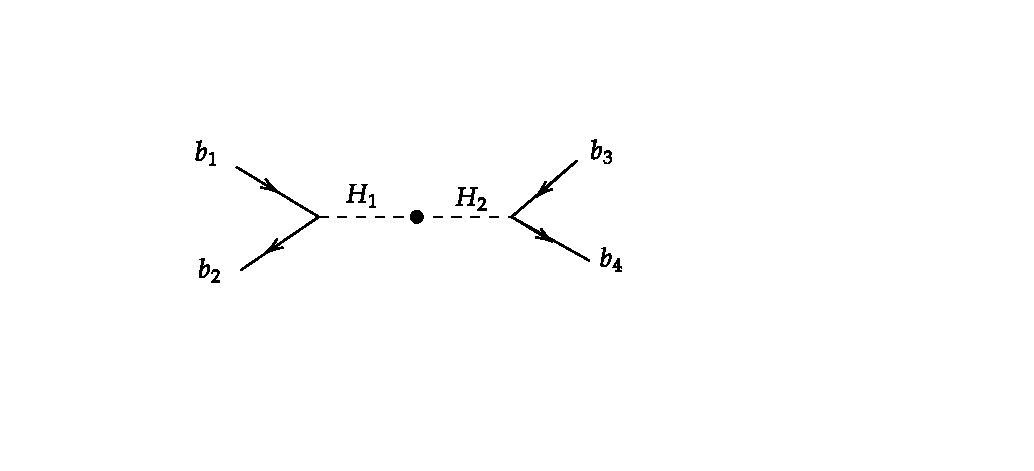
\includegraphics[width=0.5\linewidth]{Images/4.HH4b Analysis/Higgs intro/topology di-higgs.pdf}
    \caption{Topology of the $HH \to 4b$ decay}
    \label{fig: topology}
\end{figure}

In the following, the leading Higgs $H_1$ will correspond to the Higgs with the highest transverse momentum such that \pt($H_1$) > \pt($H_2$). $H_2$ will be referred to as the subleading Higgs. The leading Higgs has a mass $M_{H1}=125$ GeV while the subleading Higgs has a mass $m_{H2}=120$ GeV

\subsection{Samples} \label{subsection: samples}

The results presented in Sections \ref{section: improving} and \ref{section: s/b classification} relie on Monte Carlo (MC) simulated events (for signal and QCD multijet) as well as Run 3 2022 data. These samples are introduced in this Section. The signal events, i.e the HH production through the gluon-gluon fusion (ggHH) process are generated using \texttt{POWHEG} 2.0 and interfaced with \texttt{PYTHIA} for fragmentation and hadronization. The ggHH samples used in the following are either from:
\begin{itemize}
    \item SM official dataset, initially containing around 8M events with \kl=1
    \item \kl official dataset, initially containing around 100K events for \kl $\in \{0,2.45,5\}$
    \item \kl private datasets, initially containing 1.5M events with $\kappa_\lambda 
\in \{-2.0, -1.0, 0.0, 0.5,$ $ 1.0, 1.5, 2.0, 2.45, 3.0, 3.5, 4.0, 5.0\} $
\end{itemize}

Although in the official datasets it is possible to use samples with \kl $\in \{0,1,2.45,5\}$, the private samples are used in Section \ref{subsection: kl} as they allow to train the models for more \kl values and have significantly more statistics. Figure \ref{fig: eta h1 for validation} shows a validation study performed to ensure the validity of the private samples by comparing the distribution of observables to the distributions of the official samples. Even though Figure \ref{fig: eta h1 for validation} only shows the pseudo-rapidity $\eta$ of the leading Higgs, the validation was also performed for the following kinematic variables:

\begin{itemize}
    \item \pt, $\eta, m $ of the leading Higgs
    \item \pt, $\eta, m $ of the subleading Higgs
    \item \pt, $\eta, m, \Delta \eta_{HH}, \Delta \Phi_{HH} $ of the di-Higgs system
\end{itemize}


\begin{figure}[h!]
    \centering
    \begin{subfigure}[b]{0.4\textwidth}
        \centering
        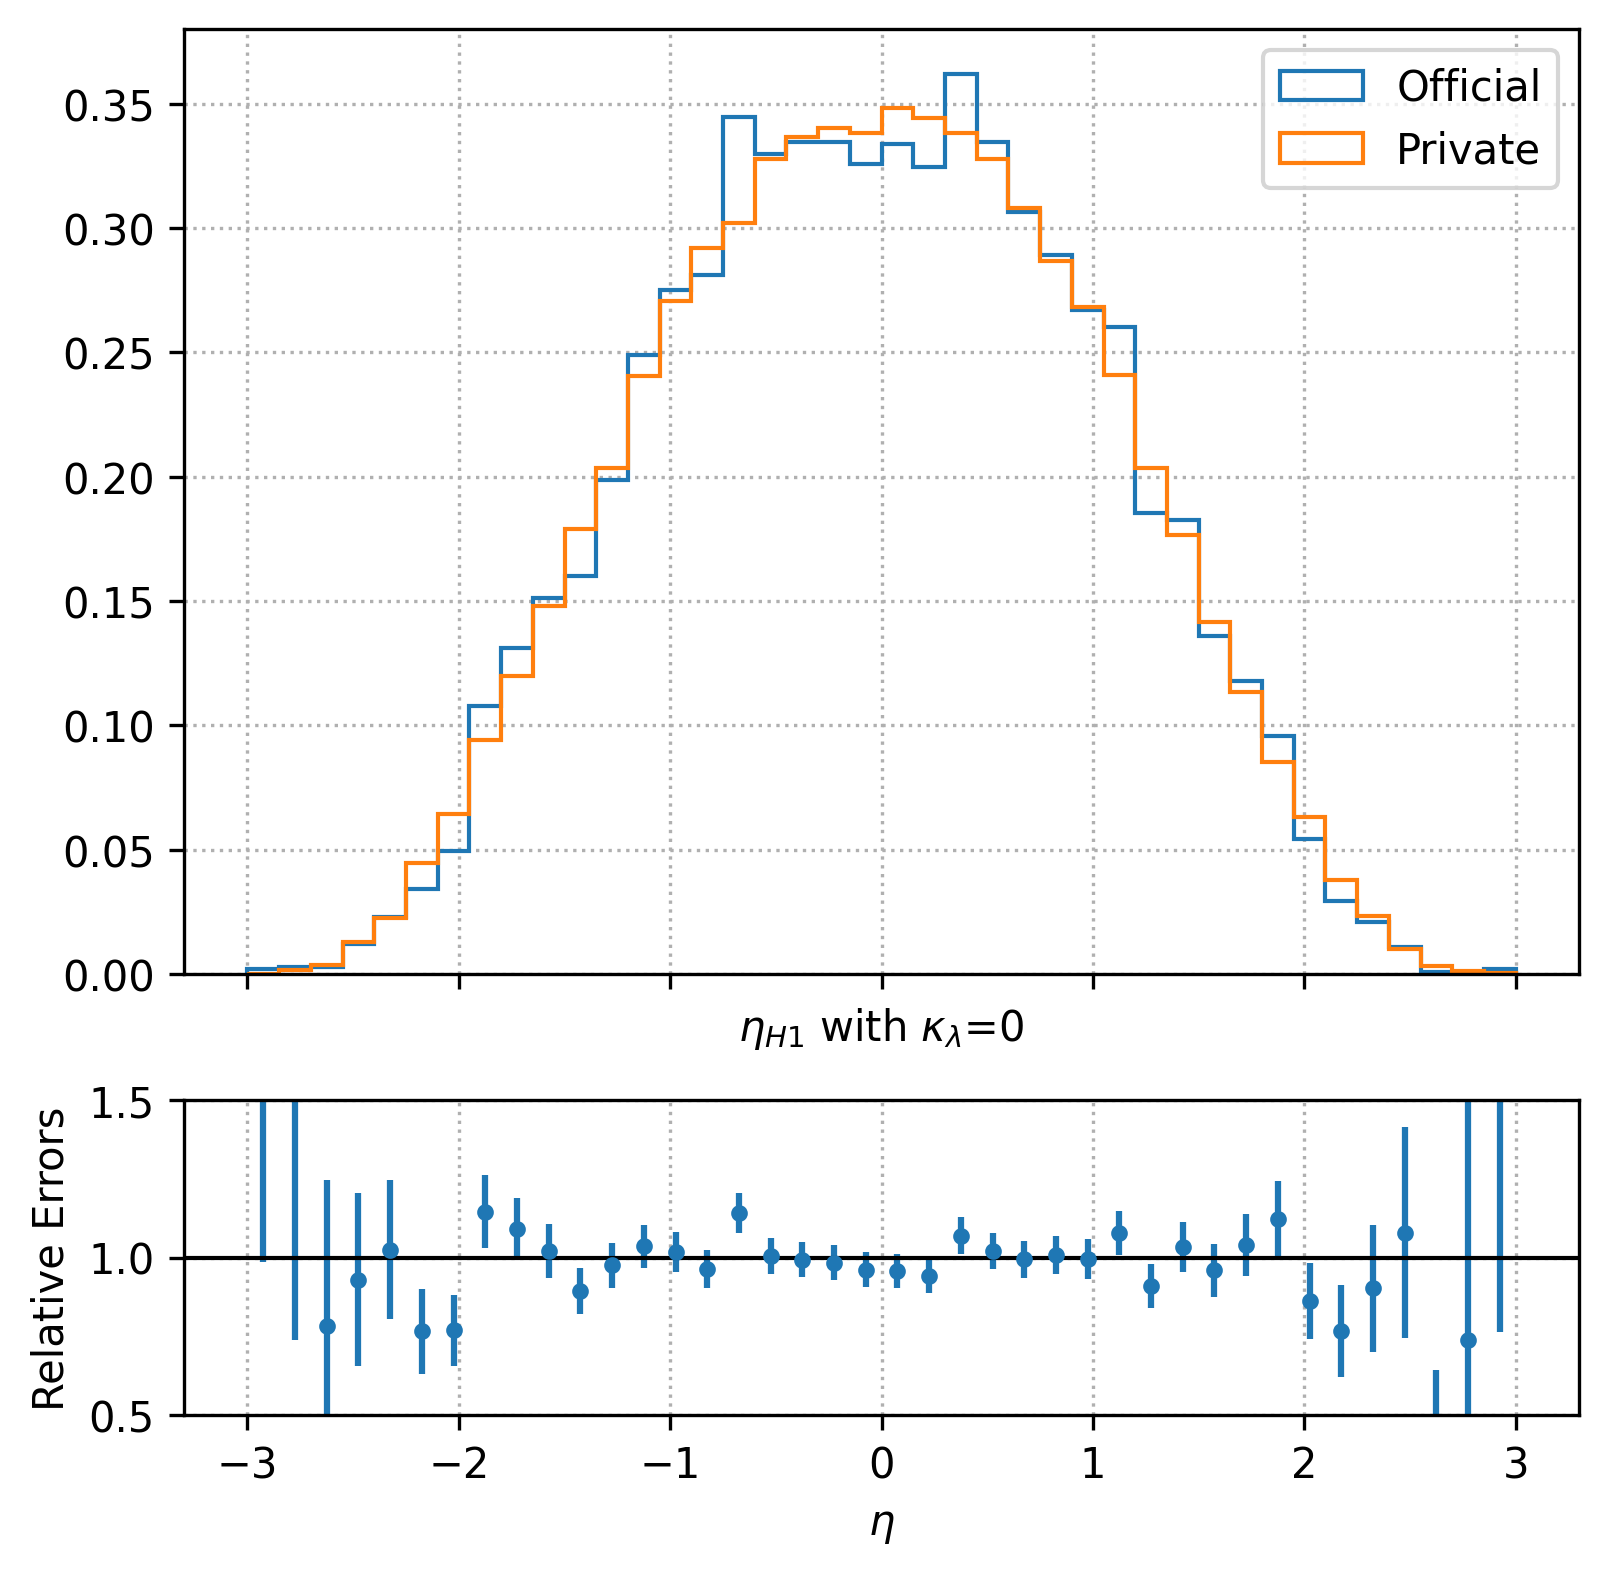
\includegraphics[width=\textwidth]{Images/4.HH4b Analysis/Validation plots/eta 0.png}
        \caption{$\eta$ of the leading Higgs for \kl=0}
        \label{fig: kl0}
    \end{subfigure}
    \hfill
    \begin{subfigure}[b]{0.4\textwidth}
        \centering
        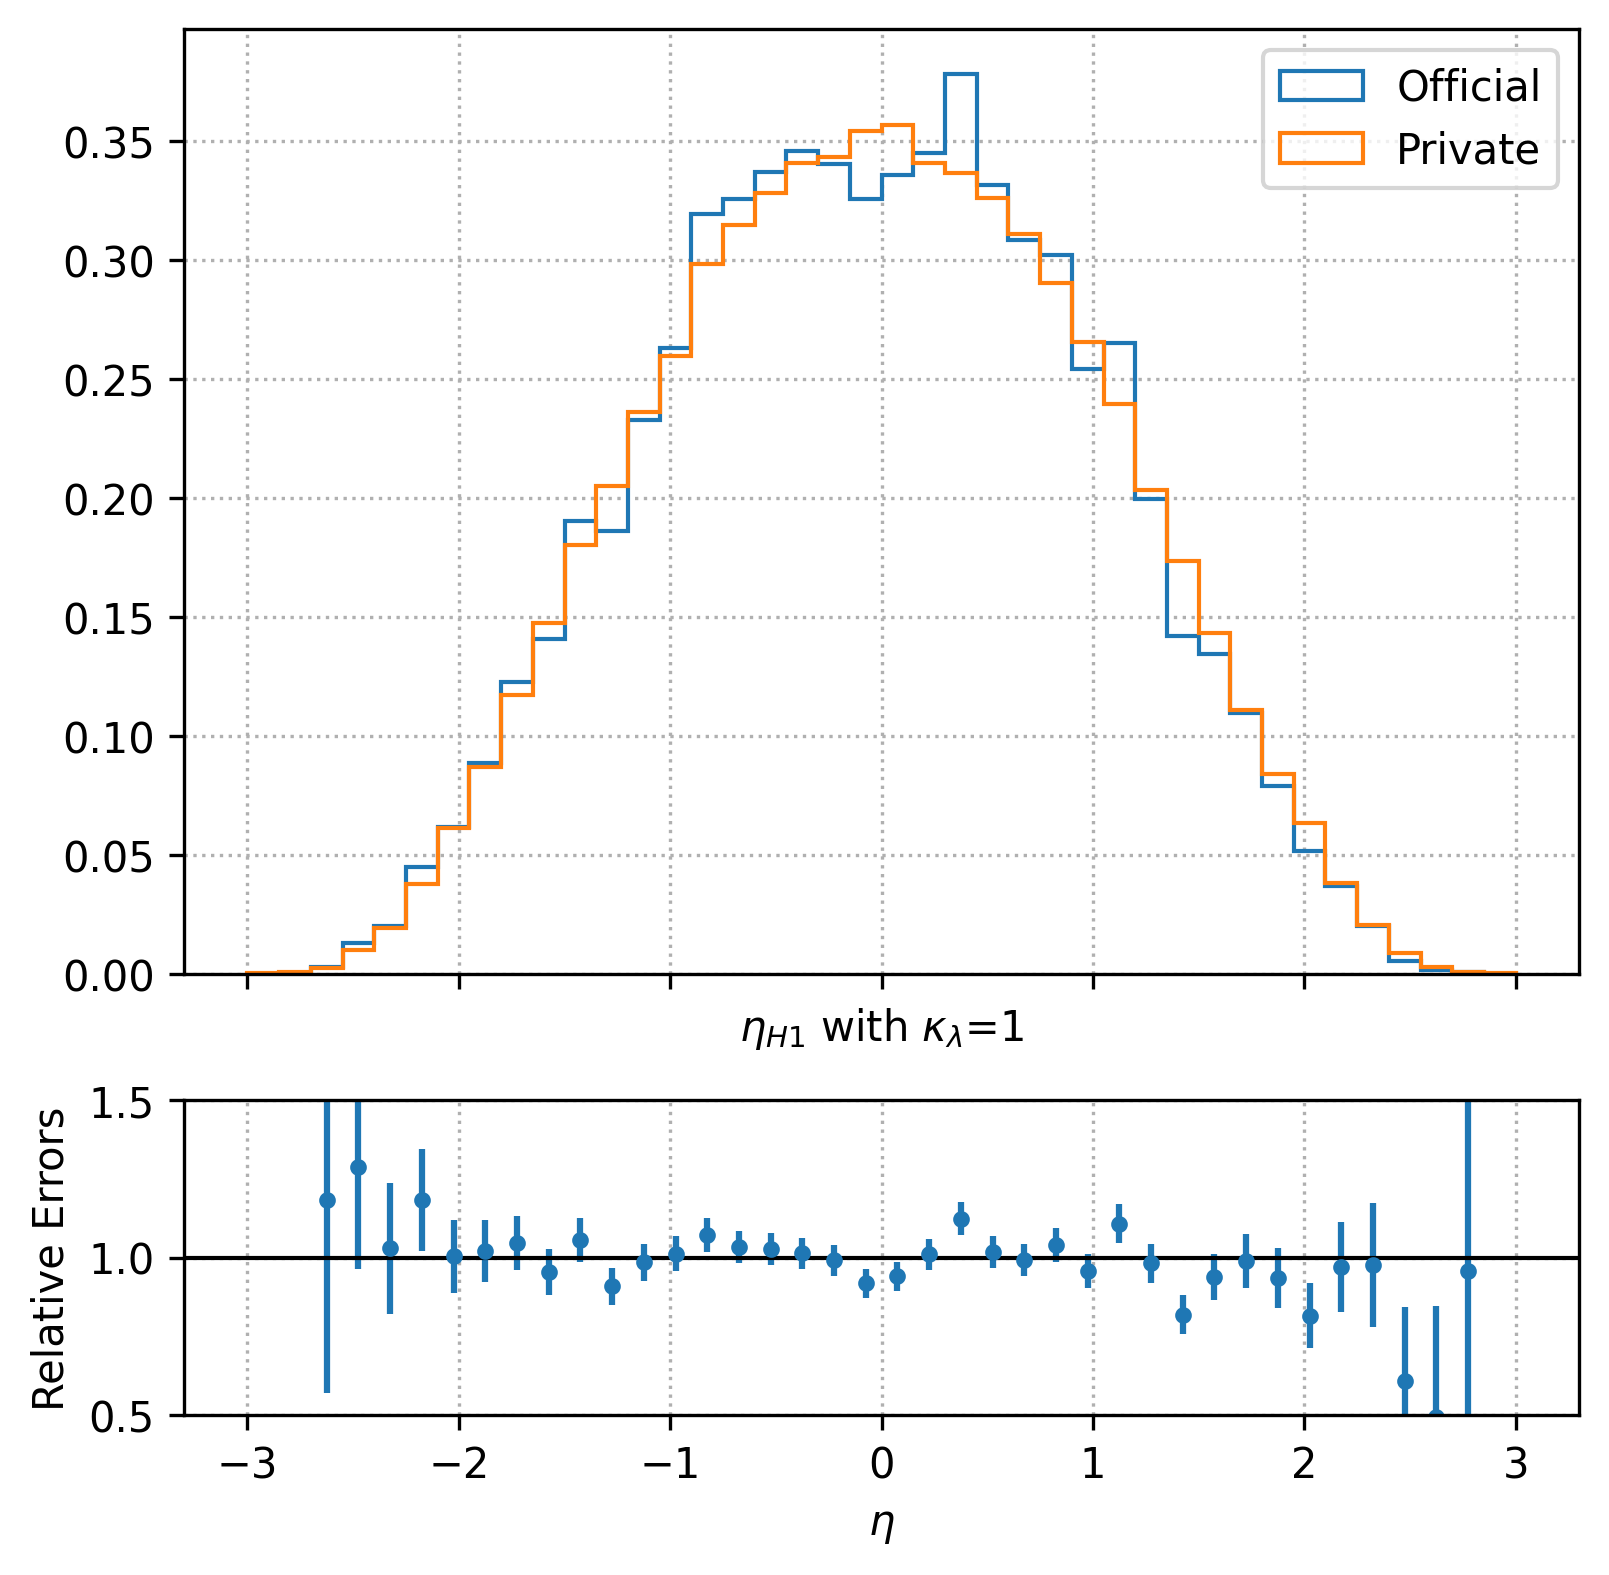
\includegraphics[width=\textwidth]{Images/4.HH4b Analysis/Validation plots/eta 1.png}
        \caption{$\eta$ of the leading Higgs for \kl=1}
        \label{fig: kl1}
    \end{subfigure}

    \vskip\baselineskip
    
    \begin{subfigure}[b]{0.4\textwidth}
        \centering
        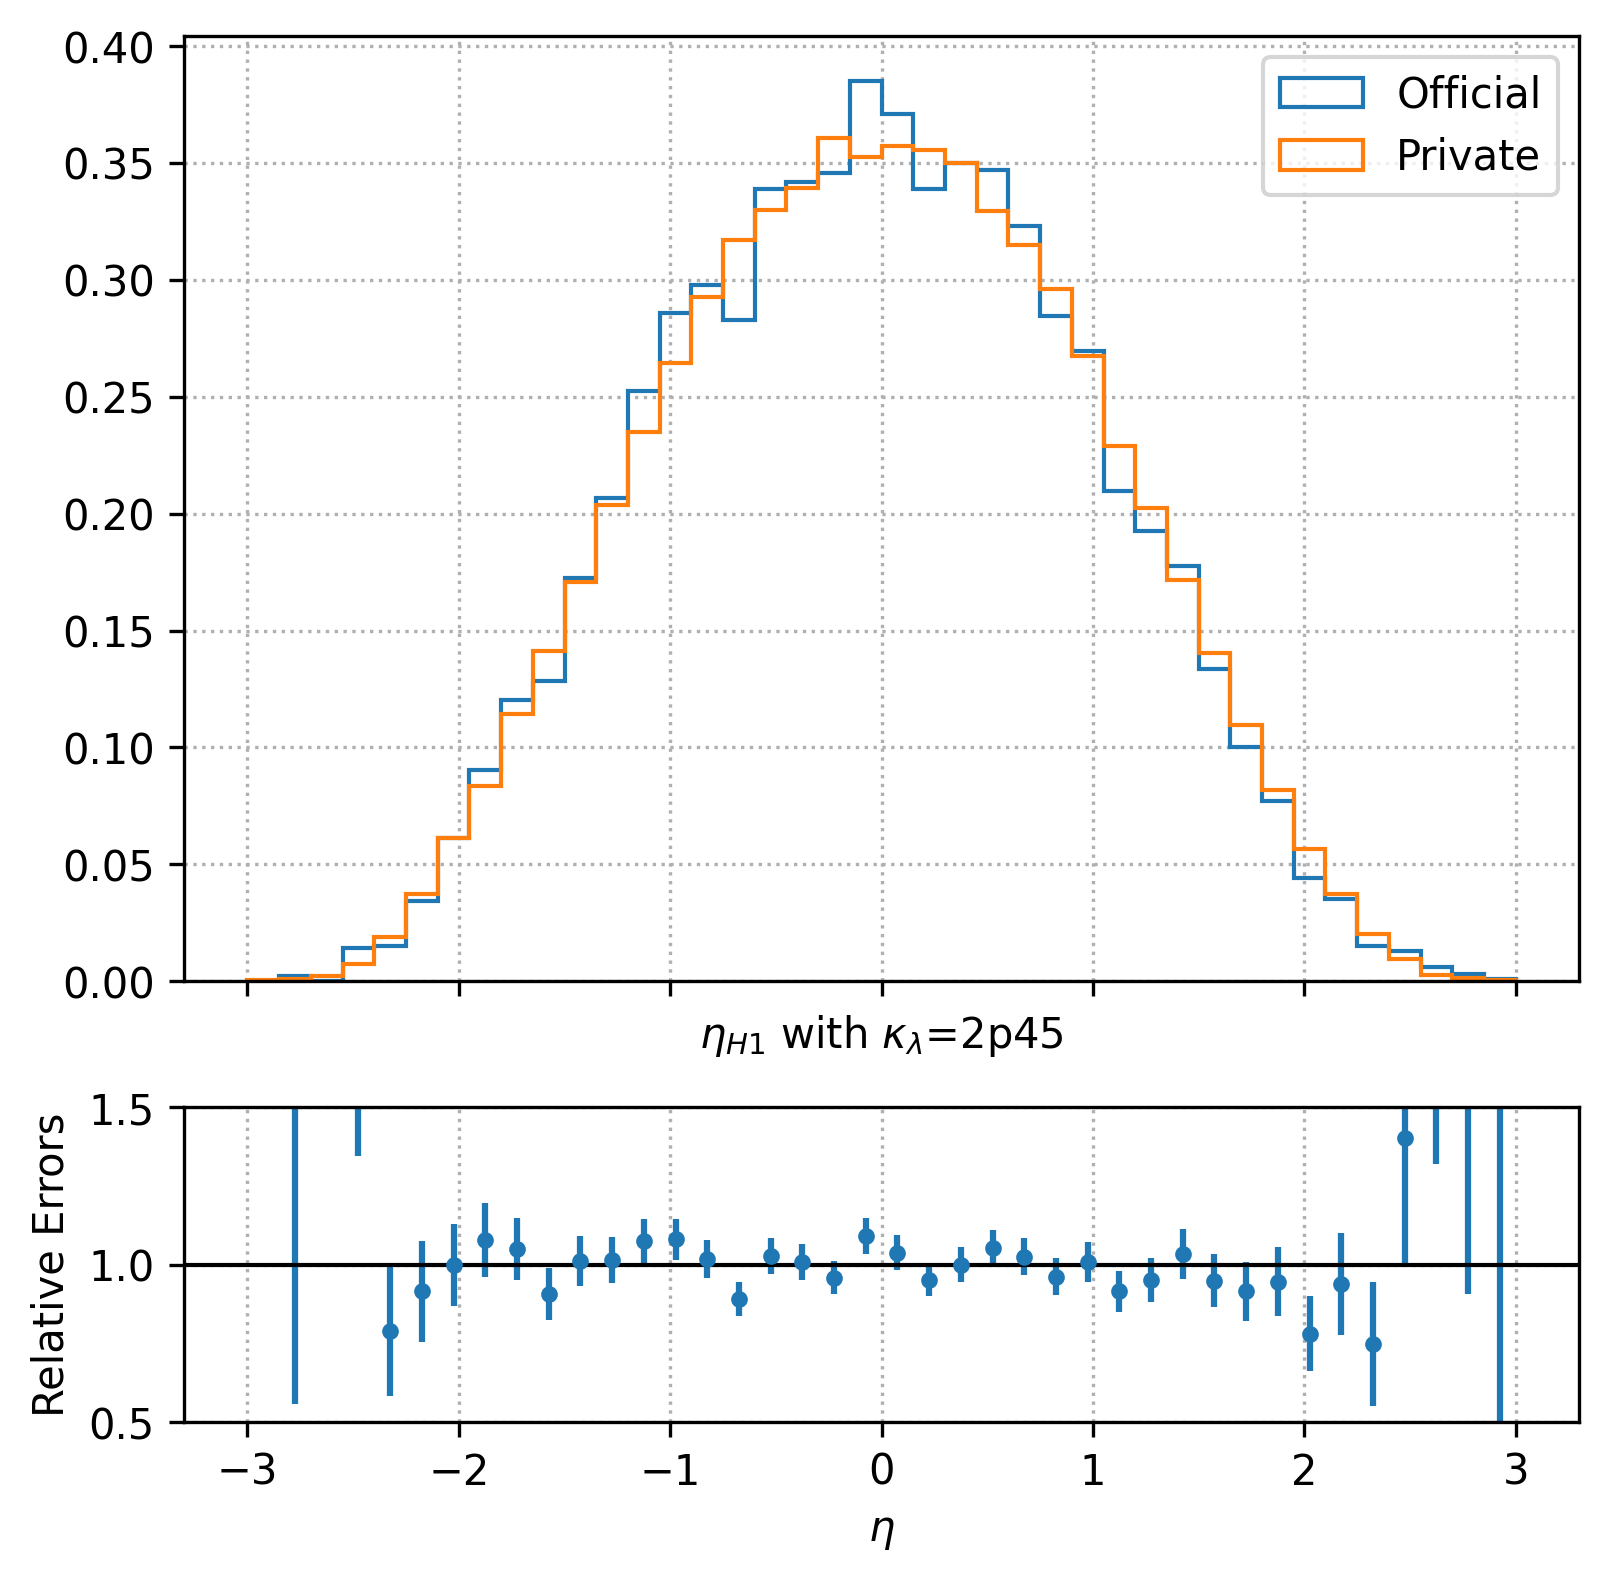
\includegraphics[width=\textwidth]{Images/4.HH4b Analysis/Validation plots/eta 2p45.png}
        \caption{$\eta$ of the leading Higgs for \kl=2.45}
        \label{fig: kl2p25}
    \end{subfigure}
    \hfill
    \begin{subfigure}[b]{0.4\textwidth}
        \centering
        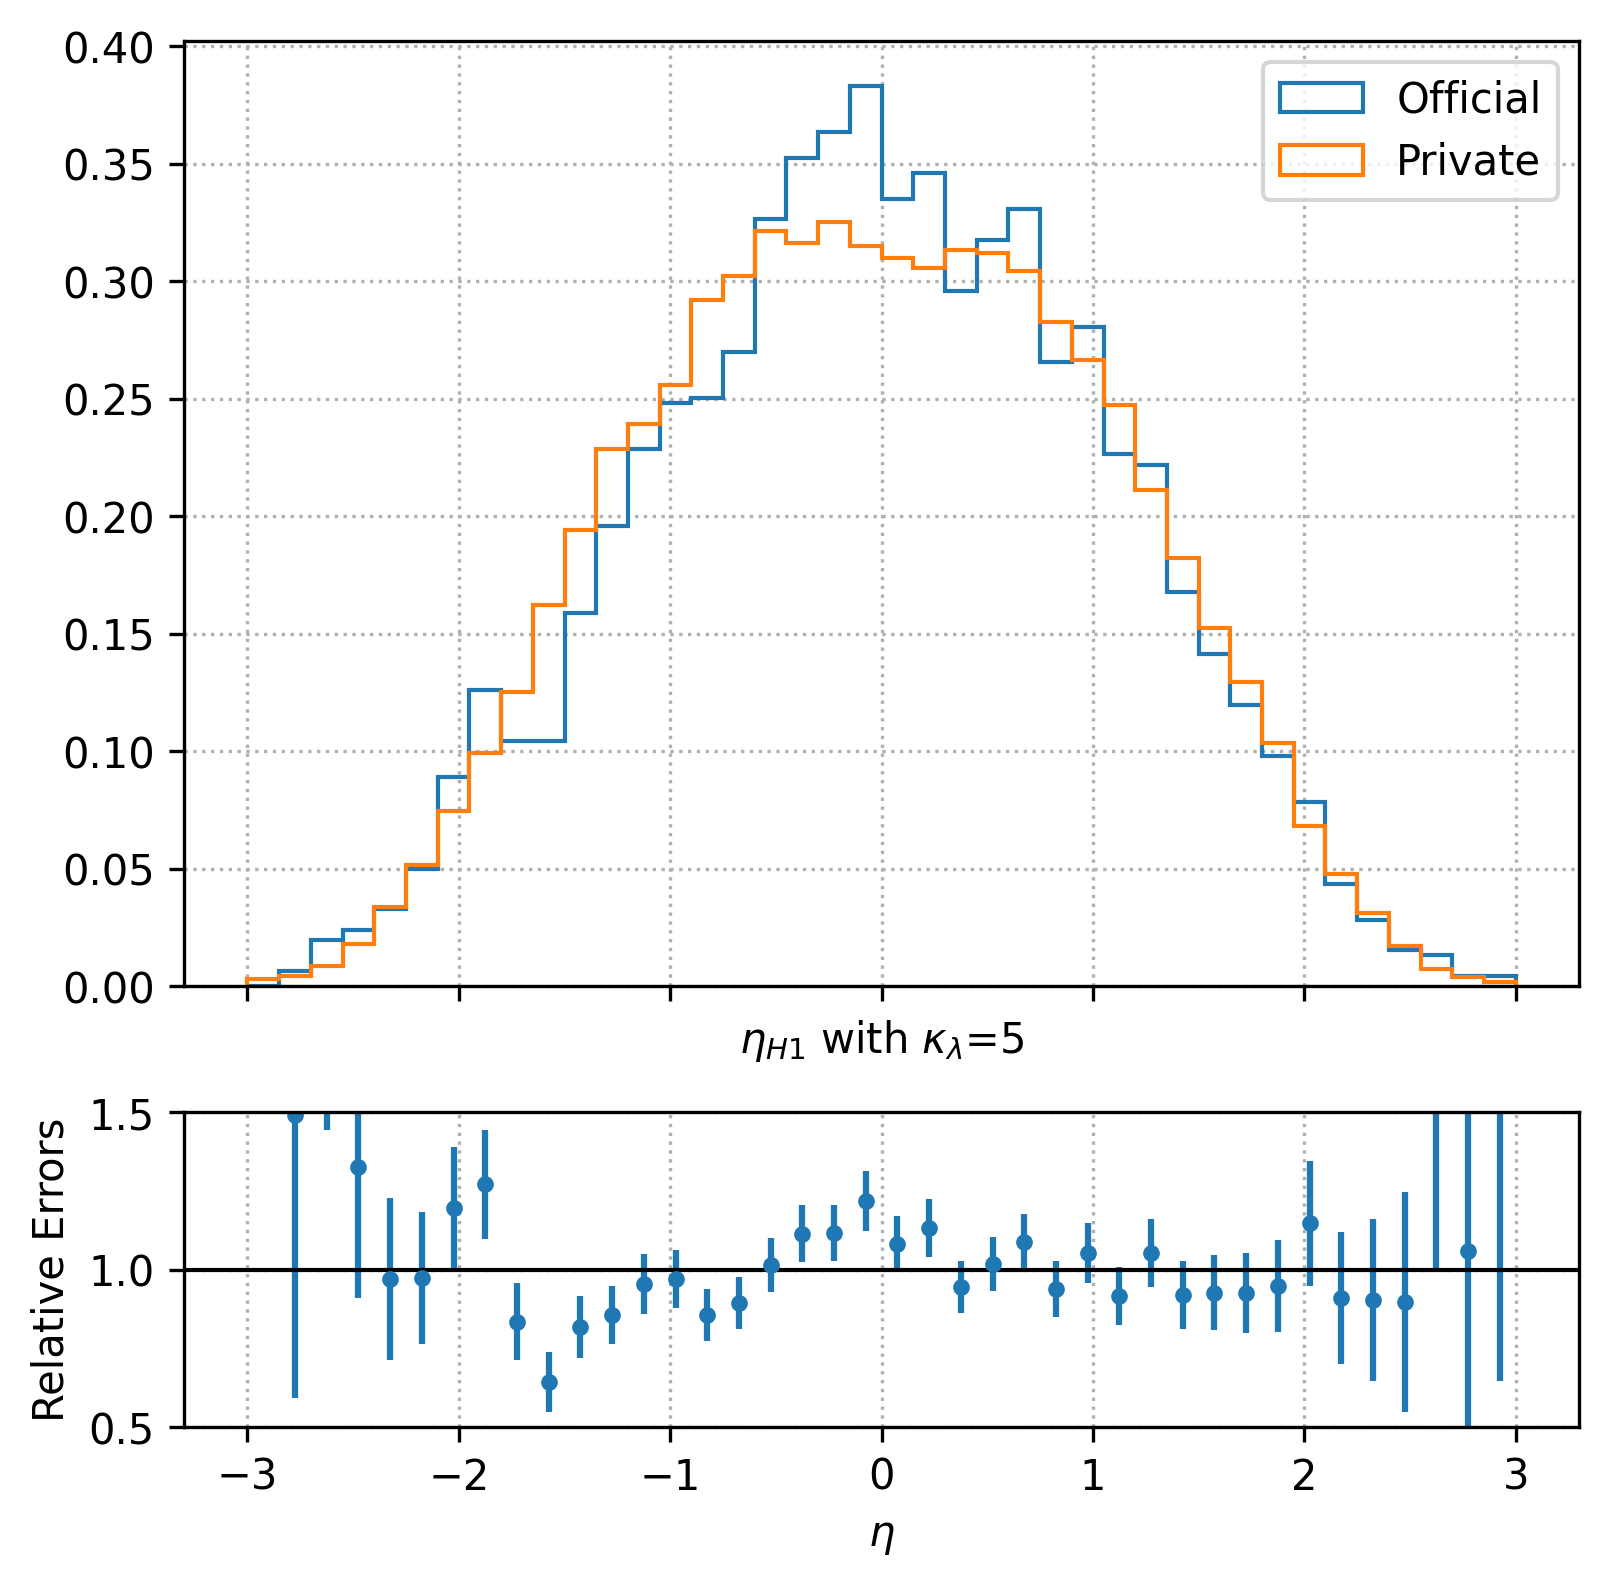
\includegraphics[width=\textwidth]{Images/4.HH4b Analysis/Validation plots/output.png}
        \caption{$\eta$ of the leading Higgs for \kl=5}
        \label{fig: kl5}
    \end{subfigure}
    
    \caption{Comparison of the $\eta$ of the leading Higgs for different \kl between the private and official signal samples}
    \label{fig: eta h1 for validation}
\end{figure}

For the HH to 4b analysis, the main background is QCD multijet. It is produced by \verb|MADGRAPH5_aMC@NLO| at leading order accuracy (LO) in the coupling constant $\alpha_s$." (cite) The jets from the matrix element calculations are matched to the parton shower produced by \verb|PYTHIA| using the MLM prescription." The QCD multijet background is produced per \Ht bins, Table \ref{table: QCD  multijet} reports the different \Ht bins and the corresponding cross-section.

\begin{table}[hbt]
    \centering
    \begin{tabular}{|c|c|c|}
        \hline
       Process  & \Ht bin [GeV] & $\sigma \times$ BR [pb] \\
       \hline
       QCD multijet in \Ht bins  & 200-400  & 1.968e+06 \\
        & 400 to 600  &  1.000e+05\\
        & 600 to 800 & 1.337e+04 \\
        & 800 to 1000 &  3.191e+03\\
        & 1000 to 1200  &  8.997e+02\\
        & 1200 to 1500 & 3.695e+02 \\
        & 1500 to 2000  & 1.272e+02 \\
        & from 2000 on  & 2.514e+01 \\
    \hline
    \end{tabular}
    \caption{\Ht bins produced for the QCD MC multijet background with the corresponding cross-section of the process per \Ht bin}
    \label{table: QCD  multijet}
\end{table}

Finally, data samples are used to test the background mass sculpting in Section \ref{subsection: bckg mass sculpting} and as background for the classification in Section \ref{section: s/b classification}. These datasets contain data collected in Run 2022 E, during Run 3. The dominant process in this data sample used as background is QCD multijet. Therefore, in the following, the background will always refer to the QCD multijet process. Nevertheless, a distinction will be made between MC-produced QCD samples (QCD MC) and data QCD samples (data) from Run 3.

\newpage

\subsection{Preselections for HH to 4b Run 3 analysis} \label{subsection:cutflows}
This section reports the characteristics of the Tight cuts used in Sections \ref{subsection: choice of inputs}, \ref{subsection: bckg mass sculpting}, \ref{subsection: kl}, \ref{subsection: pairing variability},  \ref{subsection: grid search} and the Loose cuts that are applied to the Run 3 data.

\begin{table}[hbt]
\centering
\begin{tabular}{|M{3cm}||M{12cm}|}
 \hline
 HLT  & \begin{verbatim}
    QuadPFJet70_50_40_35_PFBTagParticleNet_2BTagSum0p65
\end{verbatim} \\
 \hline
 Lepton Veto & \begin{itemize}
     \item e ($\mu$): \pt >15 (10) GeV,  $\eta$<2.4 
     \item e ($\mu$): \verb|mvaIso_WP80| (looseID)
     
     \item PF Iso $(\Delta R < 0.3) < 0.15$
     
     \item $d_{xy}$ barrel <0.05
     \item $d_{z}$ barrel <0.1
     \item $d_{xy}$ endcap <0.1
     \item $d_{z}$ endcap <0.2
 \end{itemize} \\
 \hline
 $\geq$ 4b jet candidates & \begin{itemize}
     \item \pt > 35 GeV
     \item $\eta$ < 2.5
     \item jetID with Lepton Veto
     \item No trigger matching
 \end{itemize} \\
 \hline
 HH reconstruction & \begin{itemize}
     \item 4 jets with Highest PNet b-tag score
     \item Jets ordered in \pt:
            \begin{itemize}
                \item \pt > [80,60,45,35]
            \end{itemize}
     \item Jets ordered in b-tag:
        \begin{itemize}
            \item Mean PNet of the leading 2 b-tag jets > 0.65
            \item 3° and 4° jet PNet b-tag > 0.2605 
        \end{itemize}
 \end{itemize}\\
 \hline
\end{tabular}
\caption{Tight cuts applied to the samples used for training. The trigger (HLT defined in Section \ref{section: CMS}) requirement is shown: 4 jets with \pt > [70,50,40,35] and the mean of the b-tag score of 2 of the jets to be above 0.65. Then the kinematic requirements of the four or more b jets required for the analysis are shown. Finally, the method to reconstruct the HH is specified.}
\label{table: Tight cuts}
\end{table}

\begin{table}[hbt]
\centering
\begin{tabular}{|M{3cm}||M{12cm}|}
 \hline
 HLT  & 
 \begin{verbatim}
    QuadPFJet70_50_40_35_PFBTagParticleNet_2BTagSum0p65
\end{verbatim}\\
 \hline
 Lepton Veto & \begin{itemize}
     \item e ($\mu$): \pt >15 (10) GeV,  $\eta$<2.4 
     \item e ($\mu$): \verb|mvaIso_WP80| (looseID)
     \item PF Iso $(\Delta R < 0.3) < 0.15$
     \item $d_{xy}$ barrel <0.05
     \item $d_{z}$ barrel <0.1
     \item $d_{xy}$ endcap <0.1
     \item $d_{z}$ endcap <0.2
 \end{itemize} \\
 \hline
 $\geq$ 4b jet candidates & \begin{itemize}
     \item \pt > 25 GeV
     \item $\eta$ < 2.5
     \item jetID with Lepton Veto
     \item No trigger matching
 \end{itemize} \\
 \hline
 HH reconstruction & \begin{itemize}
     \item All jets passing the preselections
     \item Jets ordered in \pt:
            \begin{itemize}
                \item \pt > [80,60,45,35]
            \end{itemize}
     \item Jets ordered in b-tag:
        \begin{itemize}
            \item Mean PNet of the leading 2 b-tag jets > 0.65
            \item 3° and 4° jet PNet b-tag > 0.2605 
        \end{itemize}
 \end{itemize}\\
 \hline
\end{tabular}
\caption{Loose cuts applied to the samples used for training. The trigger (HLT defined in Section \ref{section: CMS}) is shown, which requires 4 jets with \pt > [70,50,40,35] and the mean of the b-tag score of 2 of the jets to be above 0.65. Then the kinematic requirements of the four or more b jets required for the analysis are shown. Finally, the method to reconstruct the HH is specified.}
\label{table: Loose cuts}
\end{table}

Tables \ref{table: Tight cuts} and \ref{table: Loose cuts} outline the characteristics regarding the HLT and Lepton veto requirements when applying the Tight or Loose cuts respectively. They also report the preselections of the four or more jets considered for the pairing as well as the HH reconstruction requirements. The difference between Tight and Loose cuts is in the selections for the jets considered for the pairing and in the HH reconstruction. When applying Loose cuts, the jets are required to have a \pt > 25 GeV while for the Tight cuts the requirement is \pt > 35 GeV. Moreover, when applying the Tight cuts for the HH reconstruction only the 4 jets with the highest PNet b-tag score are considered whereas in the Loose cuts all the jets passing the preselections specified in Table \ref{table: Loose cuts} are considered. 

Applying the Tight cuts to the priavte SM signal sample (with \kl=1), containing around 8M events before preselections, leaves a sample containing around 1.7M events after preselections. Applying Loose cuts to this sample results in 2.1M events after preselections. This leads to an increase of 24\% in the number of events. Figure \ref{fig: validation cuts} shows the results of the study comparing the distributions of observables in the signal samples for different \kl. The distribution of the newly added events when considering Loose cuts, i.e. the events where at least one of the jets in the event has \pt $\in [25-35]$ GeV, is also shown. It is noticeable that when applying the Loose cuts the \pt and $m$ distributions are shifted to the left. This feature is understood by looking at the distribution of the newly added events, which have lower \pt and therefore shift the total distribution towards lower \pt and mass.

Finally, Tables \ref{table: SE kl 1}, \ref{table: SE kl 0}, \ref{table: SE kl 2p45} and \ref{table: SE kl 5} show the signal efficiency for \kl=\{ 1,0,2.45,5\} respectively. As expected, the signal efficiency is higher when the Loose cuts are applied.

\begin{figure}[h!]
    \centering
    \begin{subfigure}[b]{0.4\textwidth}
        \centering
        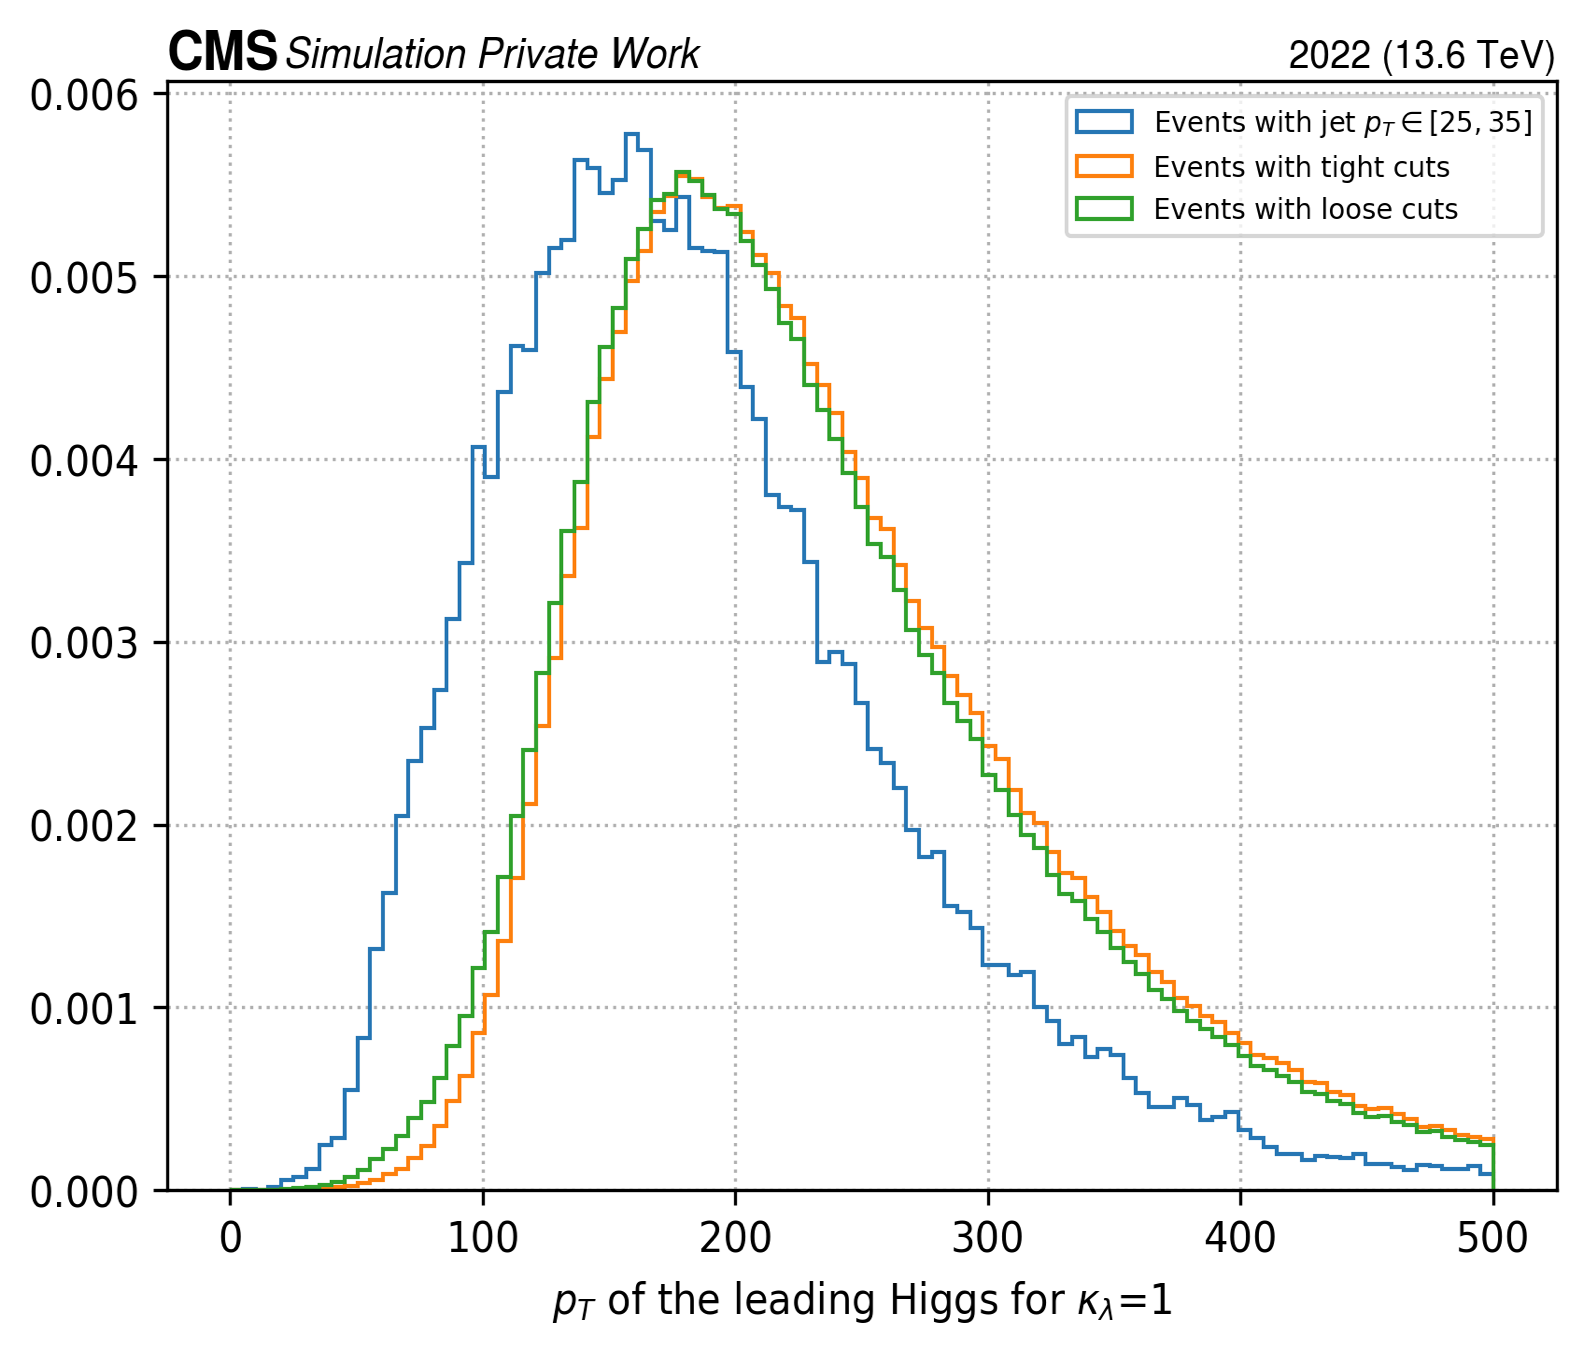
\includegraphics[width=\textwidth]{Images/4.HH4b Analysis/New events/pt h1.png}
        \caption{\pt of the leading Higgs when Loose or Tight cuts are applied to the signal sample}
        \label{fig: pt h1}
    \end{subfigure}
    \hfill
    \begin{subfigure}[b]{0.4\textwidth}
        \centering
        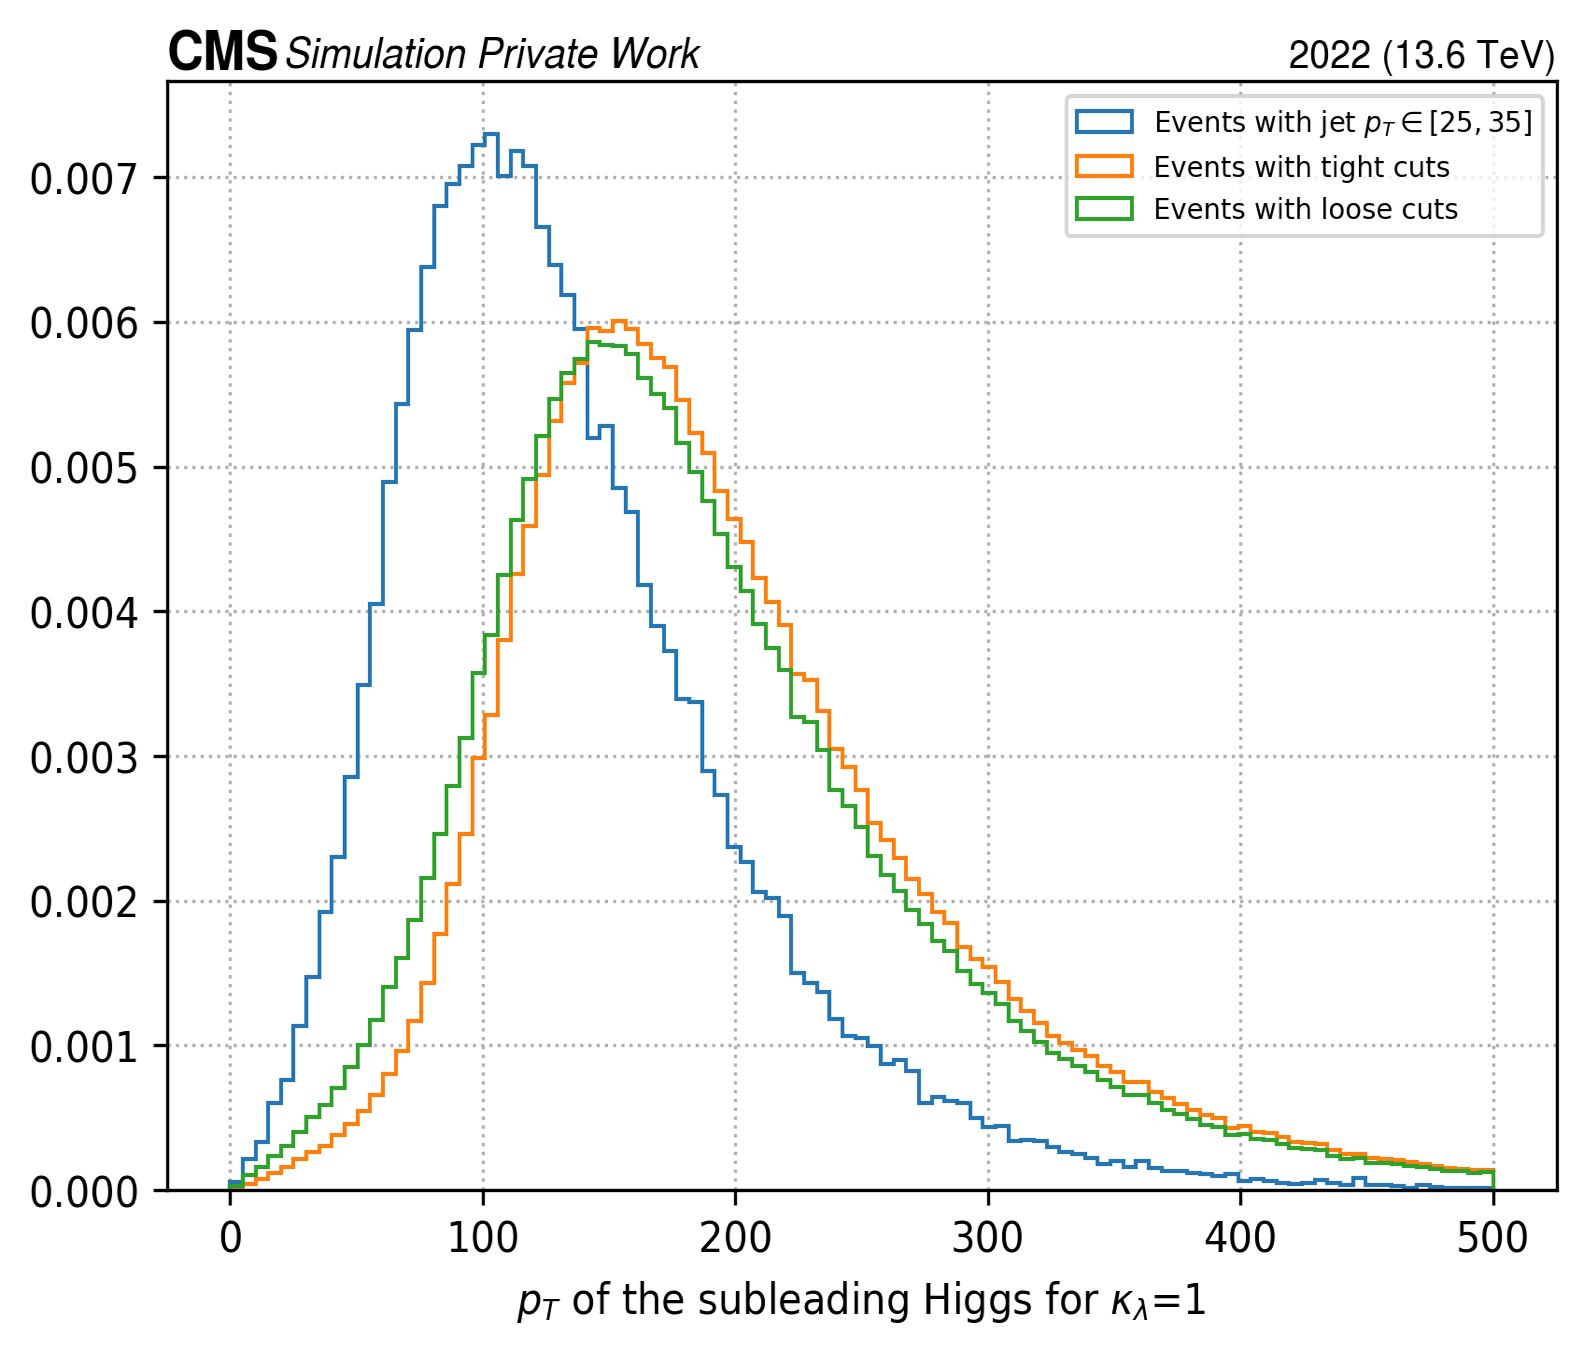
\includegraphics[width=\textwidth]{Images/4.HH4b Analysis/New events/pt h2.png}
        \caption{\pt of the subleading Higgs when Loose or Tight cuts are applied to the signal sample}
        \label{fig: pt h2}
    \end{subfigure}

    \vskip\baselineskip
    
    \begin{subfigure}[b]{0.4\textwidth}
        \centering
        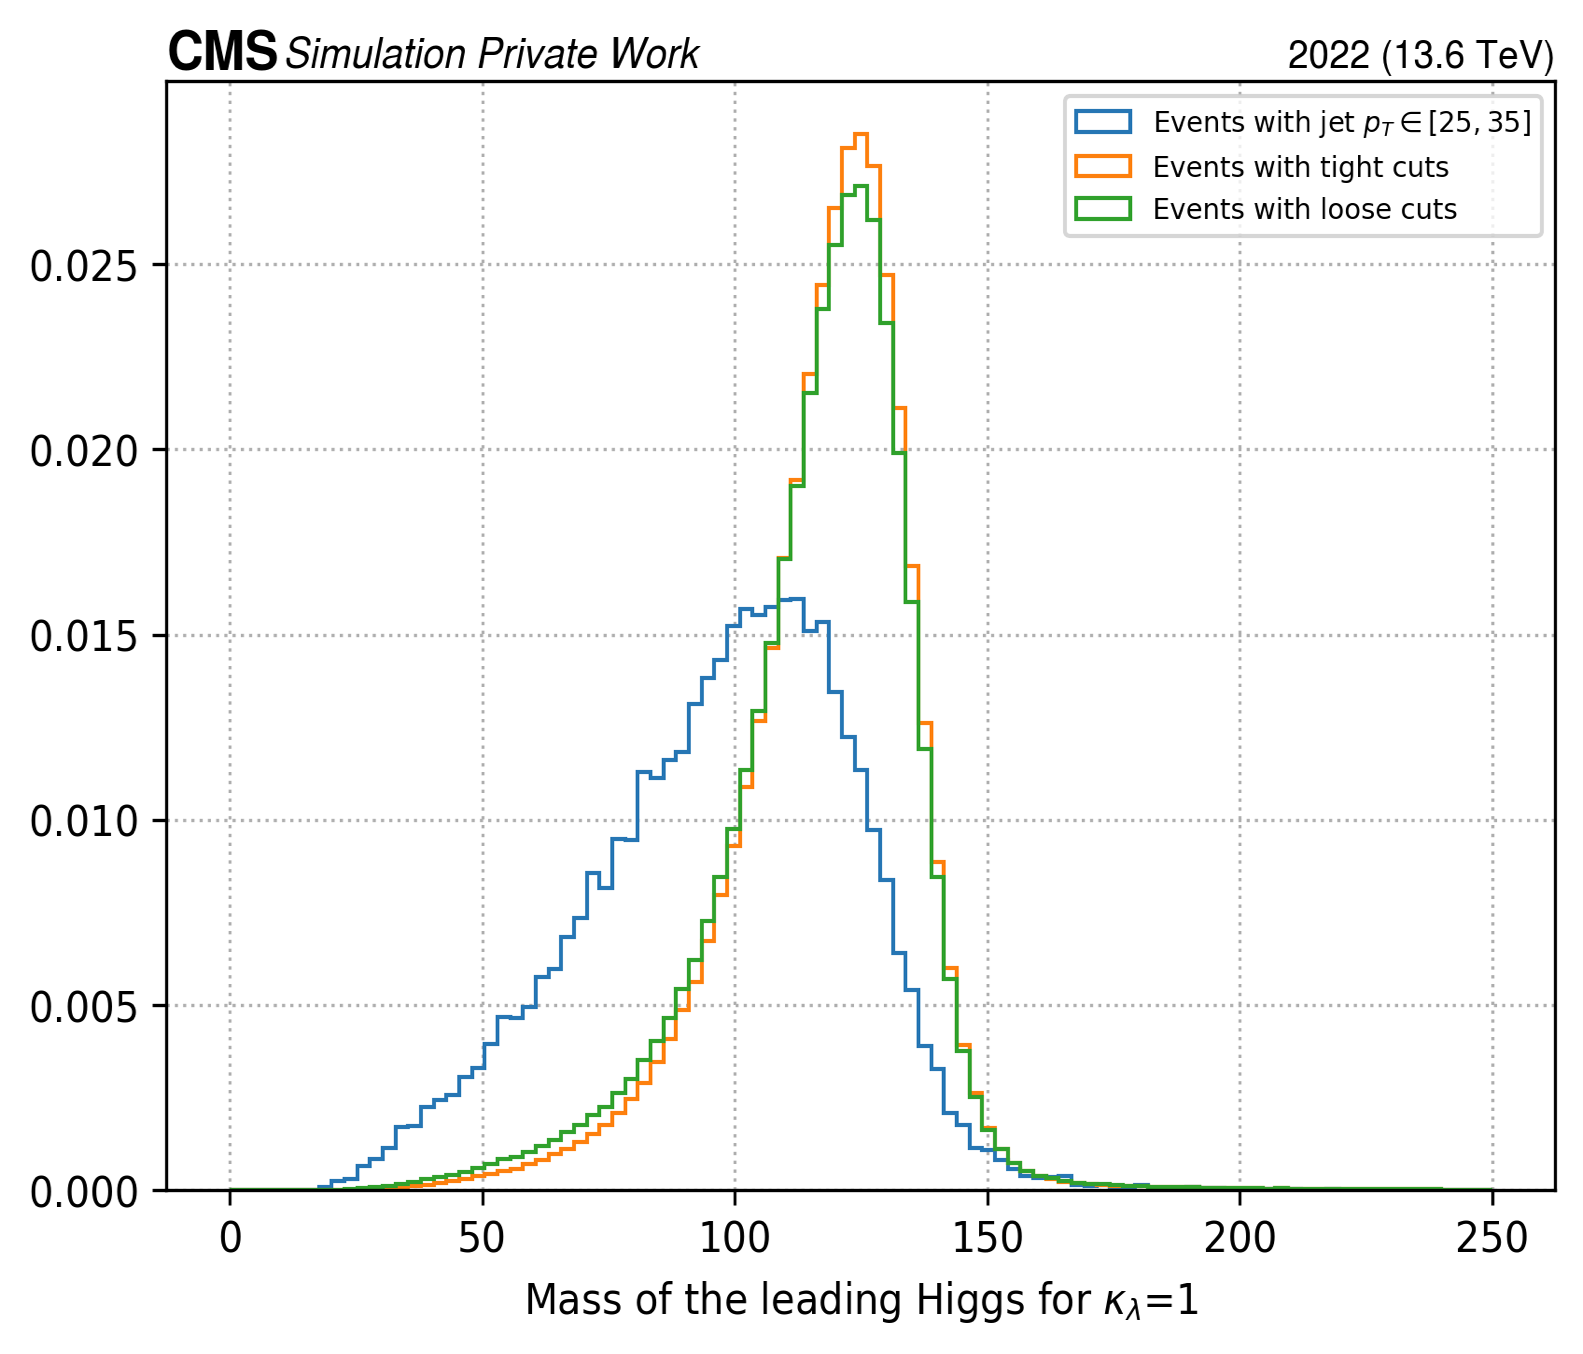
\includegraphics[width=\textwidth]{Images/4.HH4b Analysis/New events/mass h1.png}
        \caption{Invariant mass of the leading Higgs when Loose or Tight cuts are applied to the signal sample}
        \label{fig: m h1}
    \end{subfigure}
    \hfill
    \begin{subfigure}[b]{0.4\textwidth}
        \centering
        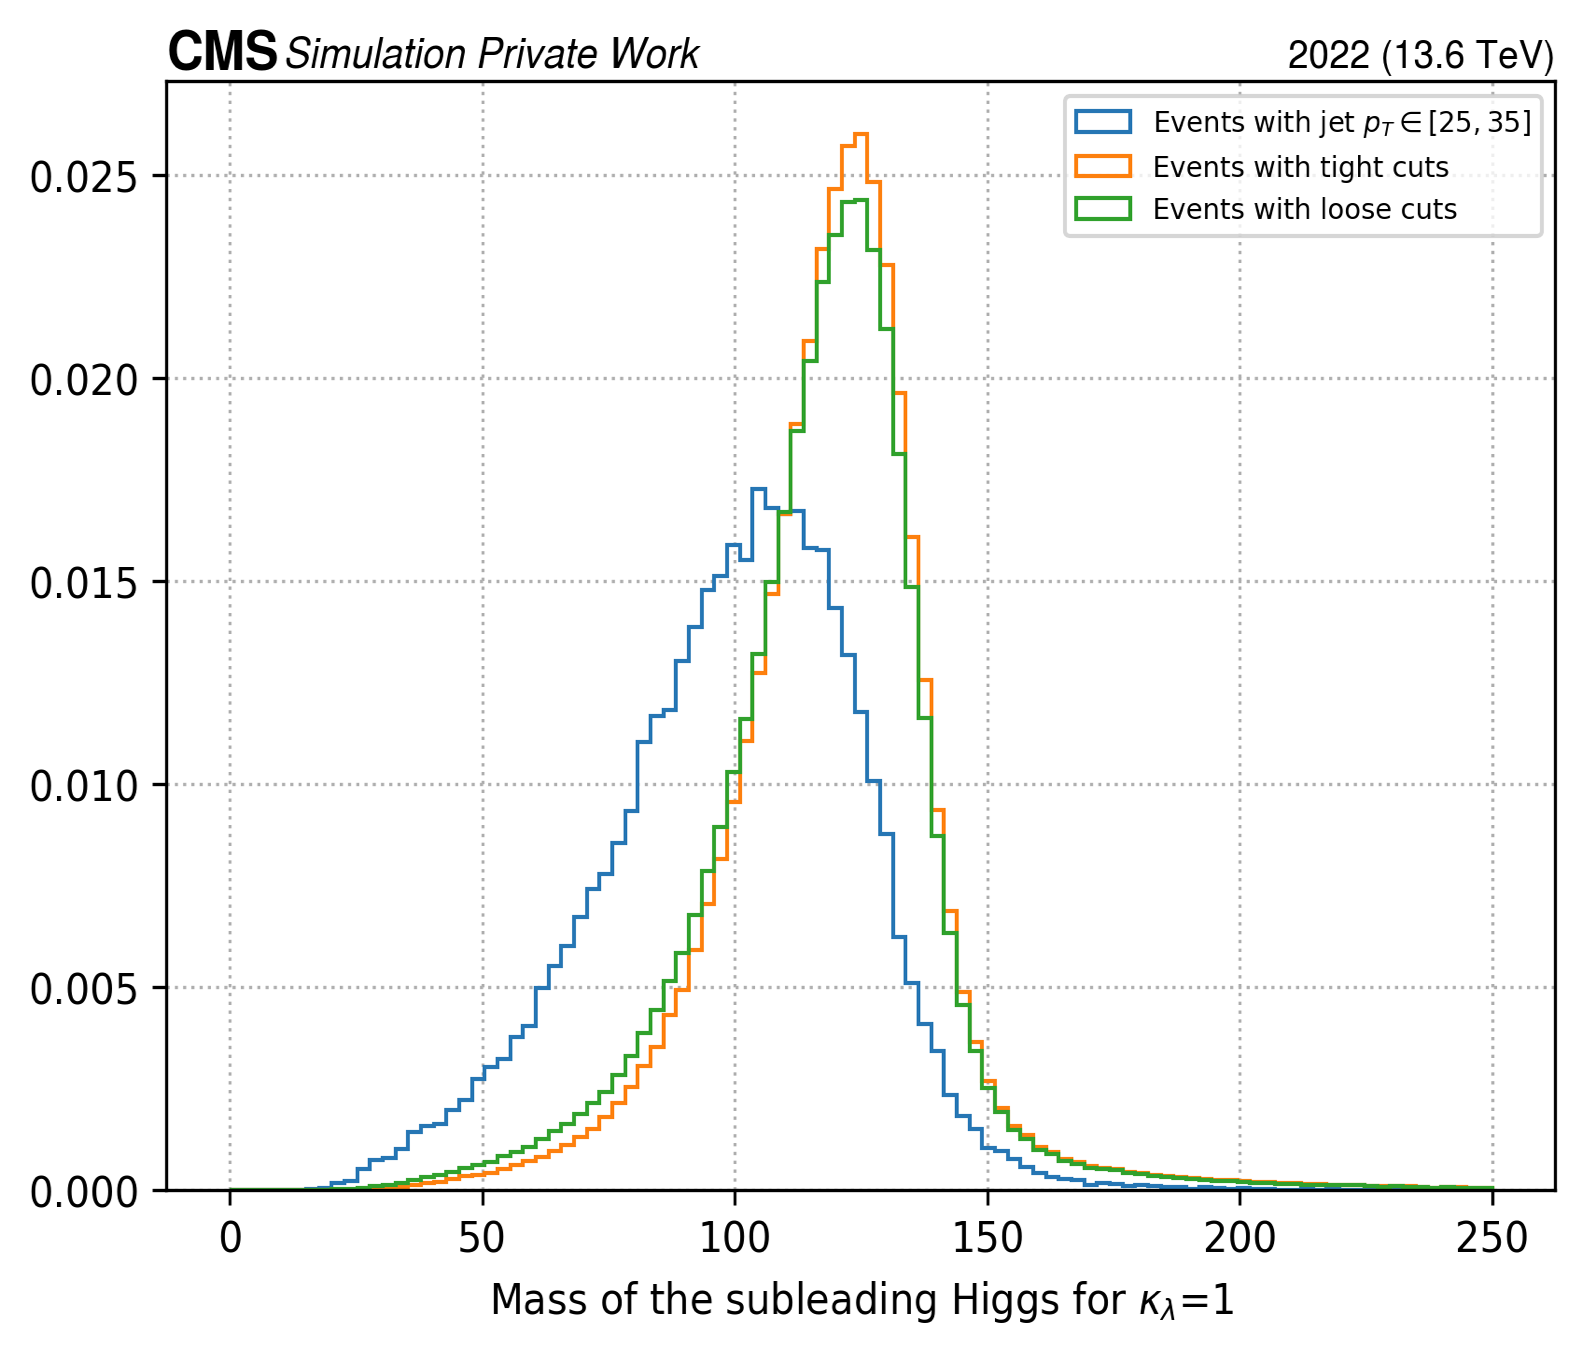
\includegraphics[width=\textwidth]{Images/4.HH4b Analysis/New events/mass h2.png}
        \caption{Invariant mass of the subleading Higgs when Loose or Tight cuts are applied to the signal sample}
        \label{fig: m h2}
    \end{subfigure}
    
    \caption{Comparison of the distribution of two different observables (\pt and $m$) of the leading and the subleading Higgs when Tight and Loose cuts are applied. The newly added events by the Loose cuts are also shown in these figures.}
    \label{fig: validation cuts}
\end{figure}

\begin{table}[hbt]
\centering
    \begin{tabular}{ |p{10cm}|p{3cm}| }
 \hline
 \multicolumn{2}{|c|}{$\kappa_\lambda$=1} \\
 \hline
 Initial number of events & 7 391 383 \\
 Signal efficiency in the 4b region with the {Tight cuts}  & 8.77 \%\\
 Signal efficiency in the 4b region with the {Loose cuts}  &  10.51 \% \\
 \hline
 \end{tabular}
\caption{Comparison of the signal efficiency when applying Loose or Tight cuts to the official sample for \kl = 1}
\label{table: SE kl 1}
\end{table}



\begin{table}[hbt]
\centering
    \begin{tabular}{ |p{10cm}|p{3cm}| }
 \hline
 \multicolumn{2}{|c|}{Private sample for $\kappa_\lambda$=0} \\
 \hline
 Initial number of events & 1 494 015 \\
 Signal efficiency in the 4b region with the Tight cuts  & 6.95 \% \\
 Signal efficiency in the 4b region with the Loose cuts  &  8.57 \% \\
 \hline
 \end{tabular}
  \caption{Comparison of the signal efficiency when applying Loose or Tight cuts to the private sample for \kl = 0}
  \label{table: SE kl 0}
\end{table}



\begin{table}[hbt]
    \centering
     \begin{tabular}{ |p{10cm}|p{3cm}| }
 \hline
 \multicolumn{2}{|c|}{Private sample for $\kappa_\lambda$=2.45} \\
 \hline
 Initial number of events & 1 489 001 \\
 Signal efficiency in the 4b region with the Tight cuts  & 9.17 \% \\
 Signal efficiency in the 4b region with the Loose cuts  &  10.92 \% \\
 \hline
 \end{tabular}
  \caption{Comparison of the signal efficiency when applying Loose or Tight cuts to the private sample for \kl = 2.45}
  \label{table: SE kl 2p45}
\end{table}


 \begin{table}[hbt]
     \centering
      \begin{tabular}{ |p{10cm}|p{3cm}| }
         \hline
         \multicolumn{2}{|c|}{Private sample for $\kappa_\lambda$=5} \\
         \hline
         Initial number of events & 1 496 012 \\
         Signal efficiency in the 4b region with the Tight cuts  & 2.81 \% \\
         Signal efficiency in the 4b region with the Loose cuts  &  4.12 \% \\
         \hline
 \end{tabular}
 \caption{Comparison of the signal efficiency when applying Loose or Tight cuts to the private sample for \kl = 5}
 \label{table: SE kl 5}
\end{table}

\subsubsection{2b and 4b regions}

Based on the multiplicity of the b-tagging jets, the datasets can be classified into regions. The 2b region requires that the mean PNet of two of the leading b-tag jets is above 0.65 and a veto is applied to the b-tag score of the third and fourth jets. This veto requires that the PNet b-tag score of the third and fourth jets be lower than 0.2605 (close to the loose WP). The 4b corresponds to the region in which either Tight or Loose cuts are applied.

Having the definitions of 2b and 4b regions, it is possible to define:
\begin{itemize}
    \item 2b data: data sample in which the requirements of the 2b region are applied
    \item 4b data: data sample in which the requirements of the 4b region are applied
    \item 2b QCD: QCD MC sample in which the requirements of the 2b region are applied
    \item 4b QCD: QCD MC sample in which the requirements of the 4b region are applied
    \item 4b signal: the signal is defined in the 4b region, therefore we will always refer to it as signal samples
    
\end{itemize}

\clearpage


\subsection{Signal and control regions}

The signal region (SR) corresponds to the region in phase space having a large signal/background (s/b) ratio. On the contrary, the control region (CR), corresponds to a region with low s/b that is close to the SR. For this analysis, a radial distance from (125,120) GeV in the $m_{H1}-m_{H2}$ is defined as follows (cite):
\begin{equation}
    R_{HH}(m_{H1}, m_{H2})=\sqrt{(m_{H1}-125)^2+(m_{H2}-120)^2}
\end{equation}
The SR is defined such that $R_{HH} < 30$ GeV and the CR such that $30 < R_{HH} < 55$ GeV


\subsection{Background estimation} \label{subsection: bckg estimation}

To estimate the background of the signal, a data-driven approach is used in this analysis due to the inadequate modeling of the QCD-induced multijet processes. This approach uses a multidimensional kinematic reweighting technique. In this case, we want to reweight the 2b data observables to match the distributions of the 4b data observables. To do so, a neural network is trained to separate CR$_{\text{2b}}$ from CR$_{\text{4b}}$ data events. the outcome of this network is the transfer function which gives the reweight factor applied to CR$_{\text{2b}}$ data to match the distributions in the  CR$_{\text{4b}}$ region. The 2b data to which we have applied these reweighting factors is the so-called "4b-morphed data".


\subsection{Presenting the pairing run 2 analysis method}

In the detector, we reconstruct at least 4 jets coming from an event signal. To identify this event as a signal event, 4 of the reconstructed jets have to be matched to the generator-level quarks. It is important to note that there are two internal symmetries to this pairing: one regarding the exchange of the $b$ quarks coming from the Higgs, as the detector can't distinguish between quark and anti-quark, and another regarding the exchange of the Higgs, it is not important the leading-\pt Higgs is associated to $H_1$ or $H_2$ in Figure \ref{fig: topology}. Therefore when considering 4 jets for the pairing (0,1,2,3), there are 3 possible combinations for the pairing, given by A, B, and C.

\begin{equation*}
   \text{Combination A}:[(0,1),(2,3)] 
\end{equation*}
\begin{equation*}
   \text{Combination B}:[(0,2),(1,3)] 
\end{equation*}
\begin{equation*}
   \text{Combination C}:[(0,3),(1,2)] 
\end{equation*}

In the Run 2 analysis, the so-called "$D_{HH}$-method" is used for the pairing. To define the goodness of the pairing with this method a distance to the diagonal in the $m_{H1}-m_{H2}$ plane is defined:

\begin{equation}
    D_{HH}=\frac{|M_{H_1}- \kappa M_{H_2}|}{\sqrt{1+\kappa^2}}
    \label{eq: dist dhh}
\end{equation}
\noindent with $\kappa=\frac{m_{H1}}{m_{H2}}=\frac{125}{120}=1.04$, accounting for the difference between the 2 Higgs masses. If the pairing is correct, it is expected that $D_{HH}$ is closer to the diagonal as shown in Figure \textbf{bla}. This distance is computed for all the possible combinations, namely $D_{HH}^A$, $D_{HH}^B$, and $D_{HH}^C$. The algorithm to choose the most successful pairing among the possible combinations is defined as follows:
\begin{itemize}
    \item The $D_{HH}$ distances are ordered from smallest to highest: $D^1_{HH}$ < $D^2_{HH}$ < $D^3_{HH}$
    \item The difference $\Delta D_{HH}= |D_{HH}^1- D_{HH}^2|$ between the two smallest distances is computed. If
        \begin{itemize}
            \item $\Delta D_{HH} > 30 GeV$ the pairing used is the one given by the combination corresponding to $D_{HH}^1$, the latter being the smallest distance.
            \item $\Delta D_{HH} < 30 GeV$ the distance (either $D_{HH}^1$ or $D_{HH}^2$) having the Higgs with the largest \pt at the center of mass frame (\pt$(H)^*$) is chosen.
        \end{itemize}
\end{itemize}

Insert figure

Figure shows the results from the Run 2 analysis using the $D_{HH}$-method for the pairing. The observed and expected 95\% confidence limits (CL) on the total cross section $\sigma_{ggF+VBF}$ HH as a function of \kl are shown. The total cross-section is defined as the sum of the ggF and VBF production modes. From these results, the observed (expected) upper limit at the 95 \% CL of the total cross-section is set to 3.9 (7.8) times the SM prediction. Moreover, the observed (expected) value of \kl is in the range -2.3 < \kl < 9.4 (-5.0 < \kl < 12.0 ) at the 95 \% CL. (cite)

Insert figure

\subsection{Classification method for Run 3 data}

For the Run 3 data, a multivariate event classifier is used to discriminate the HH to 4b signal from the QCD multijet background. The background model used for the training of the classifier is the reweighted 2b data or 4b-morphed data that is defined in Section \ref{subsection: bckg estimation}.

\vspace{1 cm}

In the following sections, the use of the attention-based neural network SPANet is proposed to determine the best pairing of jets and as a classifier to discriminate the HH to 4b signal from the QCD multijet background. The goal of SPANet is to outperform the efficiency of the $D_{HH}$-pairing method used in Run 2 as well as the performance of the classification of the multivariate event classifier used for partially Run 3 data introduced in cite by using SPANet.
